\documentclass{scrartcl}
\usepackage{amsmath}
\usepackage{amssymb}
\usepackage[geometry]{ifsym}
\usepackage{graphicx}
\usepackage[outputdir=build]{minted}

\newcommand{\selection}{\sigma}
\newcommand{\projection}{\pi}
\newcommand{\rename}{\rho}
\newcommand{\join}{\mathbin{\text{\begin{tiny}\textifsym{|><|}\end{tiny}}}}
\newcommand{\fullouterjoin}{\mathbin{\text{\begin{tiny}\textifsym{d|><|d}\end{tiny}}}}
\newcommand{\leftouterjoin}{\mathbin{\text{\begin{tiny}\textifsym{d|><|}\end{tiny}}}}
\newcommand{\rightouterjoin}{\mathbin{\text{\begin{tiny}\textifsym{|><|d}\end{tiny}}}}
\newcommand{\semijoin}{\mathbin{\text{\begin{tiny}\textifsym{|><}\end{tiny}}}}
\newcommand{\groupby}{\Gamma}

\newcommand{\mtt}[1]{\text{\texttt{#1}}}

\setlength{\parindent}{0pt}

\begin{document}

\section*{Exercise 2}

We chose the following queries for the TPC-H dataset:

\begin{listing}[H]
    \begin{minted}[autogobble]{sql}
        select *
        from lineitem l, orders o, customer c, nation n, region r
        where
            l.l_orderkey = o.o_orderkey and
            o.o_custkey = c.c_custkey and
            c.c_nationkey = n.n_nationkey and
            n.n_regionkey = r.r_regionkey
    \end{minted}
    \caption{Query 1}
\end{listing}

\begin{listing}[H]
    \begin{minted}[autogobble]{sql}
        select *
        from region r, nation n, supplier s, partsupp ps, part p
        where
            r.r_regionkey = n.n_regionkey and
            n.n_nationkey = s.s_nationkey and
            s.s_suppkey = ps.ps_suppkey and
            ps.ps_partkey = p.p_partkey and
            r.r_name = 'EUROPE' and
            p.p_size = 12
    \end{minted}
    \caption{Query 2}
\end{listing}

\begin{listing}[H]
    \begin{minted}[autogobble]{sql}
        select *
        from customer c, supplier s, nation n, region r,
             lineitem l, orders o, partsupp ps, part p
        where
            c.c_nationkey = n.n_nationkey and
            s.s_nationkey = n.n_nationkey and
            n.n_regionkey = r.r_regionkey and
            c.c_custkey = o.o_custkey and
            o.o_orderkey = l.l_orderkey and
            l.l_partkey = ps.ps_partkey and
            l.l_suppkey = ps.ps_suppkey and
            ps.ps_partkey = p.p_partkey and
            ps.ps_suppkey = s.s_suppkey and
            r.r_name = 'EUROPE' and
            o.o_shippingpriority = 0 and
            l.l_linenumber = 1
    \end{minted}
    \caption{Query 3}
\end{listing}

\section*{Exercise 3}

The following graphs show the cost distribution of the picked trees:

\begin{figure}[H]
    \centering
    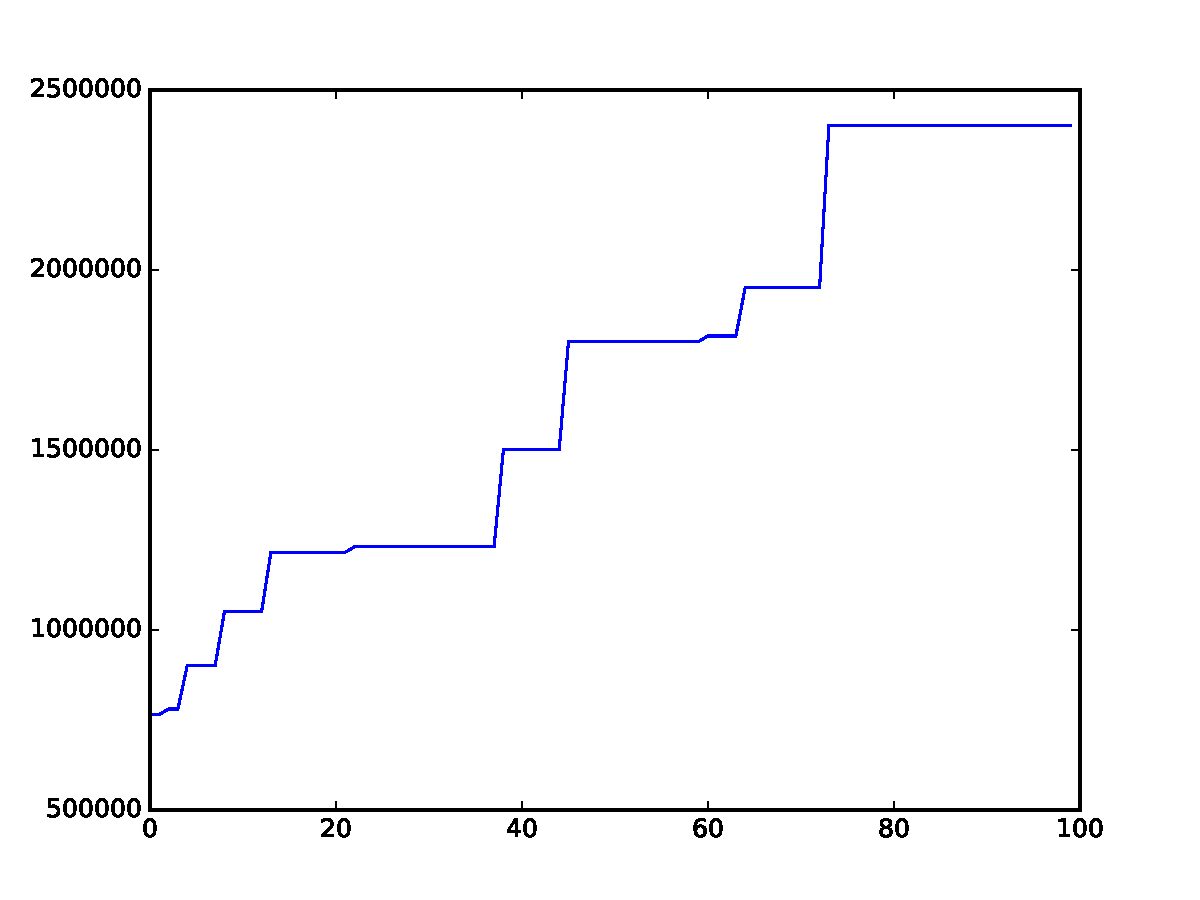
\includegraphics[scale=0.8]{plot-q1}
    \caption{Distribution for Query 1}
\end{figure}

\begin{figure}[H]
    \centering
    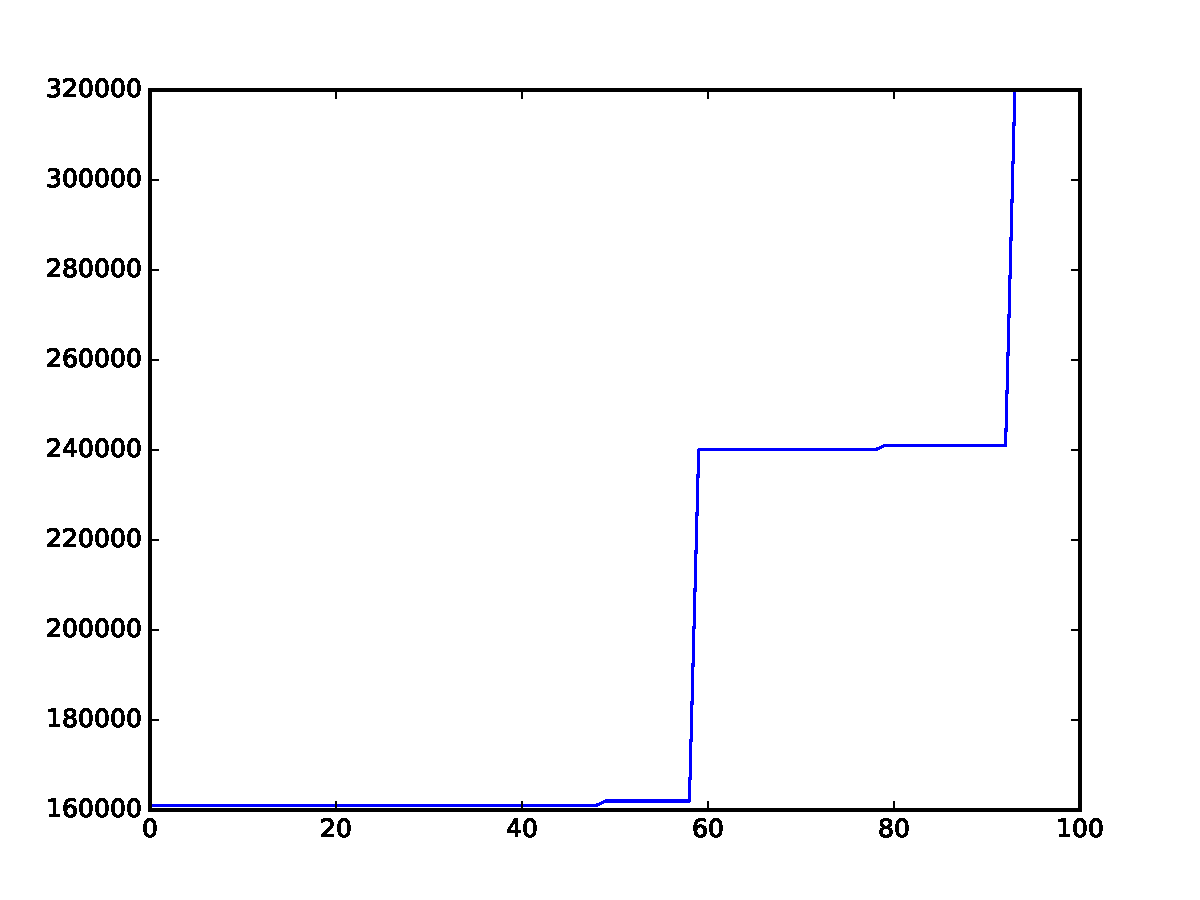
\includegraphics[scale=0.8]{plot-q2}
    \caption{Distribution for Query 2}
\end{figure}

\begin{figure}[H]
    \centering
    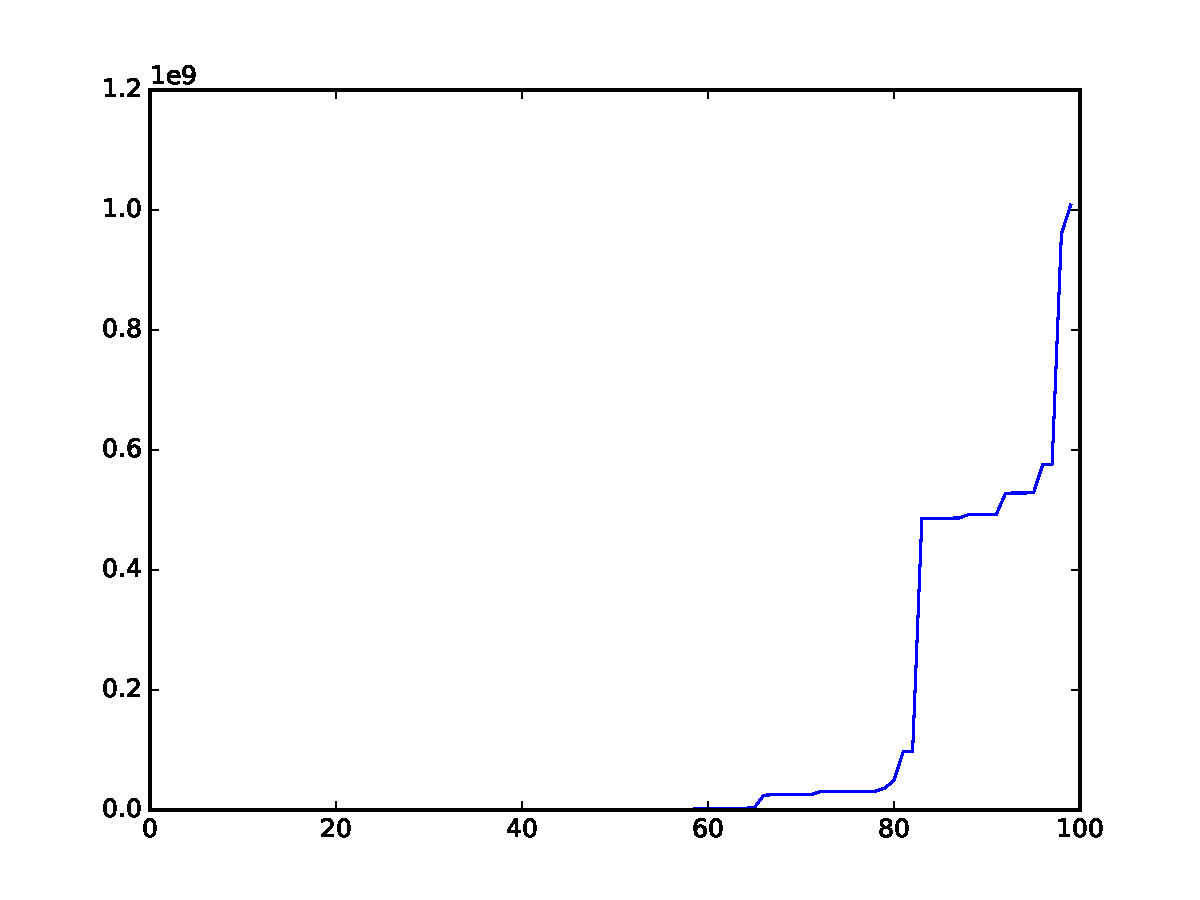
\includegraphics[scale=0.8]{plot-q3}
    \caption{Distribution for Query 3}
\end{figure}

\end{document}
